\chapter{Protein Structure}
\label{chapter:protein_structure}

\begin{quote}
``Protein engineering is not only a promising path, but it provides a very compact and (I think) persuasive argument for being able to build molecular machines, because proteins are molecular machines.'' \\ 
--- \textit{K. Eric Drexler}
\end{quote}


\section{Proteins in Nature}

Protein molecules form the major active components in the biological systems of all kingdoms of life. These polypeptides, almost exclusively composed of only  20 natural amino acids, must fulfil many essential, intricate and diverse roles; interacting together in the vast network that is the typical cell. How these polymers fulfil  their various roles in such a crowded and heterogeneous environment, whether in structure, transportation, catalysis, or regulation, is a direct consequence of the native conformation -- the three-dimensional shape that each given polypeptide adopts. A full understanding of this native state and its subsequent prediction will have a profound effect on many fields related to modern molecular biology; ultimately facilitating countless advances.
Such benefits include the \abinitio\ design of protein catalysts for industry, development of novel therapeutic small molecules and  insight into the result of genetic mutations. Many such genetic mutations are important as they yield  mis-folded or functionally altered proteins, which are implicated in a multitude of disease states.


\subsection{Protein Structure}

Chemically, an amino acid is formed from a central \al-carbon (\ca) surrounded by an amino group, a carboxyl group, a hydrogen atom and one of 20 naturally occurring \sidechains\ (figure \ref{fig:intro:aminoa}). Protein chains themselves are linear un-branched polymers of these amino acids,
formed by a series of condensation reactions; which in turn yield rigid and planar amide groups spanning the boundary between individual
amino acids. The sequence of  amino acids defines a given proteins' primary structure.

\begin{figure}[hptb]
\begin{center}
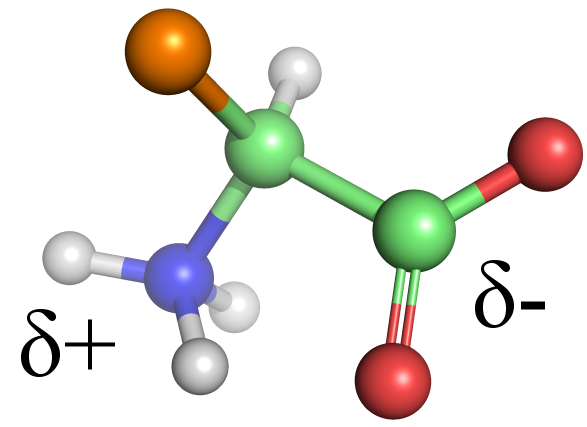
\includegraphics[width=0.40\textwidth]{./01-ProteinStructure/aminoacid/aminoacid.png}
\caption[An amino acid]{An amino acid. The R-group, which is variable between different amino acid types, is shown as a unified orange sphere. The net partial charges of the zwitterion
are shown in black text.}
\label{fig:intro:aminoa}
\end{center}
\end{figure}

The primary structure in turn dictates the formation of more complex secondary
and super-secondary structures. The core of globular proteins, which is compact and hydrophobic in nature, can be conceptually divided into  secondary structure elements which are stabilised by regular hydrogen bonding networks. Connecting these secondary elements are so-called ``random coil'' regions, also know as loops, which are intrinsically less regular
and more hydrophilic in nature.

Tertiary structure describes the association of these secondary elements. Longer single-polypeptide chains commonly form distinct globular
units termed domains, usually of around 100 amino acids in length. Domains are conserved throughout evolution both in terms of sequence and structure. It is their replication, mutation and recombination that
is thought to play a key role in driving the evolutionary process\cite{NATIVE:SUPERFAMILY:2007}. 

Finally, although not applicable to all proteins, quaternary structure describes the inter-relation of multiple polypeptide chains
 in the formation of protein complexes. These complexes can range in size from protein dimers totalling less than 150 amino acids to huge macromolecular complexes totalling many thousands of amino acids.



\subsection{The Native State} 

It is experimentally observed that denatured globular
proteins spontaneously refold into their native state once physiological
conditions are restored. This observation has the implication that the primary sequence of a polypeptide chain alone ultimately dictates its tertiary structure. The native fold represents an energetically stable structure on the hugely rugged folding landscape, postulated by the thermodynamic hypothesis to be the state with the lowest free energy\cite{NATIVE:Anfinsen1973}. The ability to predict this structural state from the polypeptide sequence alone is a central problem in molecular biology today, and is termed the
protein-folding problem. 

Despite a wealth of research, the problem of how the
chain folds into a single native conformation in the face of seemingly infinite conformational possibilities, is still poorly understood. The Levinthal paradox\cite{NATIVE:Levinthal1968} theorises that kinetic pathways for protein folding must exist, as it is estimated that a purely random conformational search of a \mer{100} polypeptide would take $10^{29}$ years\cite{NATIVE:Dobson1998}. 

By contrast, it is clear that the vast majority of naturally occurring proteins do spontaneously fold reliably and quickly into their native state, despite the astronomical number of possible conformations. They must, therefore, satisfy both a kinetic requirement for folding on an appropriate timescale and a thermodynamic requirement for a single stable folded conformation. The Levinthal paradox
is potentially
resolved by the concept that folding is guided by the rapid formation of local interactions, which then determine the further folding of the peptide. This suggests that local stretches of polypeptide form stable interactions and serve as nucleation points in the folding process.
 

Attempts to tackle the protein folding problem lie at the crossroads between the many avenues of science including biology, chemistry, physics, mathematics, statistics and computer science. Inroads towards greater understanding of native protein structure will result in more successful prediction of the native state
which will ultimately have many far reaching benefits.










\section{Protein Anatomy}

If the native state is to be predicted, it is critical that one has a clear picture of
the structural motifs that are found in globular proteins. This section illustrates common structural classifications and defines their major
features. 
\subsection{The Protein Backbone}
\label{section:intro:prot_backbone}

The polypeptide backbone can be well described in torsional space using just two backbone angles per residue, phi ($\Phi$) and psi ($\Psi$) (figure \ref{fig:intro:bb_torsion}).
The peptide group is a planar unit with a delocalised electronic structure and therefore inherently inflexible, owing to its partially double-bonded character. This  causes the Omega (\Omg) angle of the peptide group to usually lie very close to 180\degree\ corresponding to its trans-isomer, only very occasionally occupying 0\degree\ corresponding to the more sterically strained cis conformation (figure \ref{fig:intro:cis_trans}). 

\begin{figure}[hptb]
\begin{minipage}[b]{0.47\linewidth}
\centering
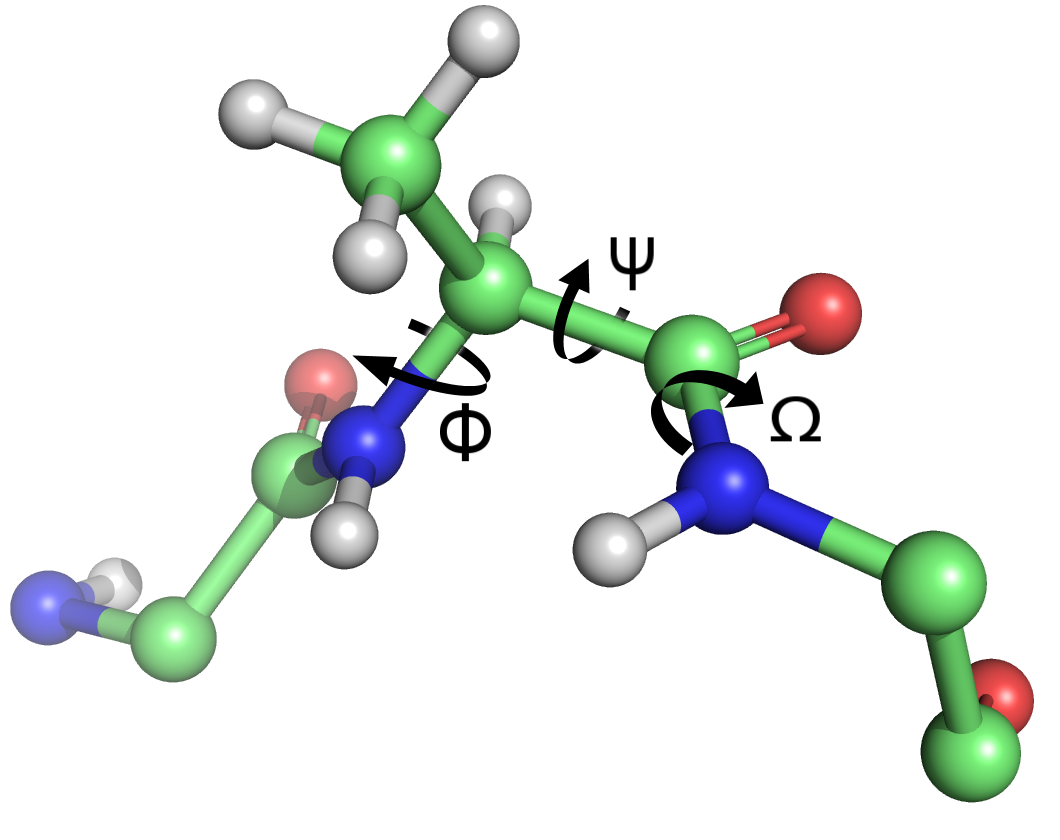
\includegraphics[width=1.0\textwidth]{01-ProteinStructure/structure/bb_torsion.png}
\caption{Protein backbone torsions.}
\label{fig:intro:bb_torsion}
\end{minipage}
\hspace{0.5cm} % To get a little bit of space between the figures
\begin{minipage}[b]{0.47\linewidth}
\centering
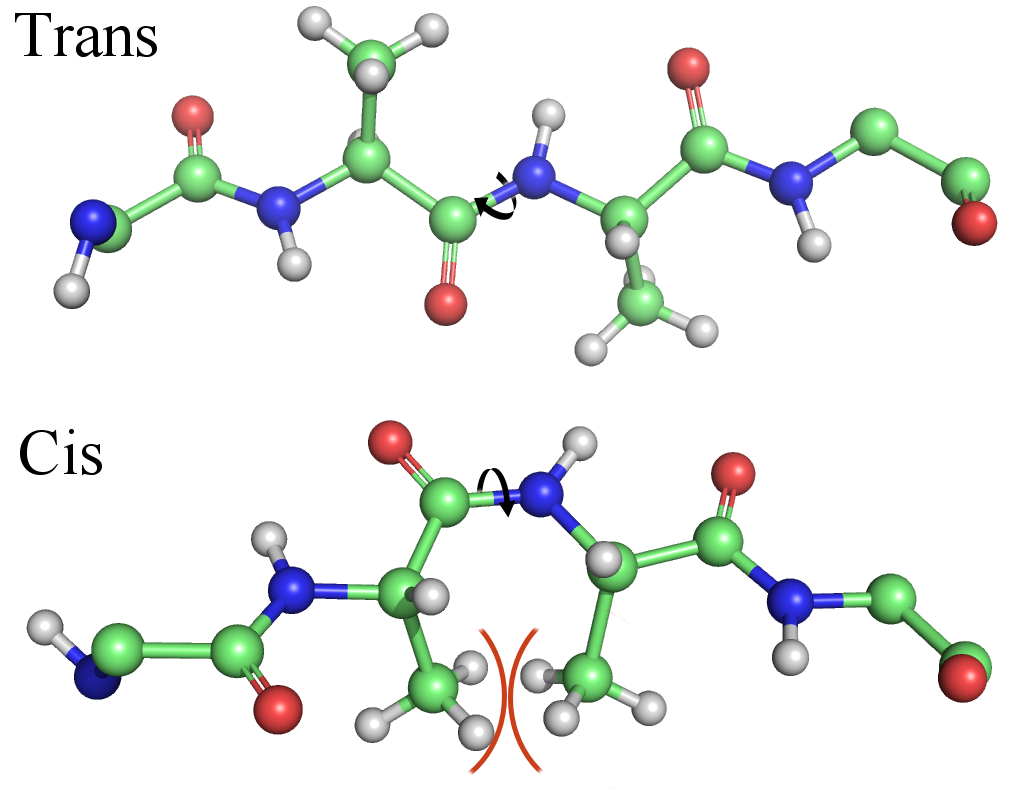
\includegraphics[width=1.0\textwidth]{01-ProteinStructure/structure/cis_trans.png}
\caption{The cis and trans-peptide group conformations.}
\label{fig:intro:cis_trans}
\end{minipage}
\end{figure}

\subsection{Amino Acid  \Sidechains}

Each of the 20 naturally occurring amino acids is defined by its  \sidechain. The major classes of these include   small, hydrophobic, nucleophilic, amide,
acidic, basic and aromatic residues. Figure \ref{fig:intro:chi} shows the bonds that are available for rotation, which are commonly annotated with the letter $\chi$ and numbered
away from the central \mainchain\ \ca-atom. The exact number of possible $\chi$-angles is obviously dependent on the residue. 


\begin{figure}[hptb]
\begin{center}
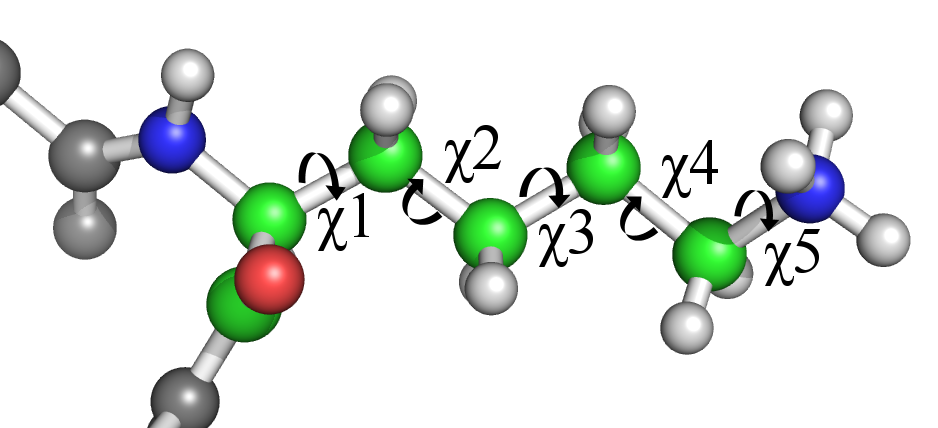
\includegraphics[width=0.6\textwidth]{01-ProteinStructure/sidechain/chi.png}
\caption{The \sidechain\ $\chi$ torsions of lysine.}
\label{fig:intro:chi}
\end{center}
\end{figure}

\Sidechain\ $\chi$-angles can be used to describe the rotational states  of the \sidechain. Following clustering of the the \sidechain\ conformations within the PDB, distinct conformational classes can be defined. Libraries of these commonly populated states, termed rotamer libraries\cite{NATIVE:Kan93,NATIVE:Dun97,NATIVE:Shetty2003}, are available for use in protein modelling.


\subsection{The Ramachandran Plot}
\label{section:intro:ramachandran}

Residue backbone conformations are generally visualised by the using a Ramachandran plot\cite{NATIVE:Ramachandran1963,NATIVE:Ramachandran1968} (Figure \ref{fig:intro:ramachandran}), which plots the values of the \phipsi\ backbone torsional angles against each other and in which regions of high population density can clearly be seen. 

\begin{figure}[hptb]
\begin{minipage}[b]{0.47\linewidth}
\centering
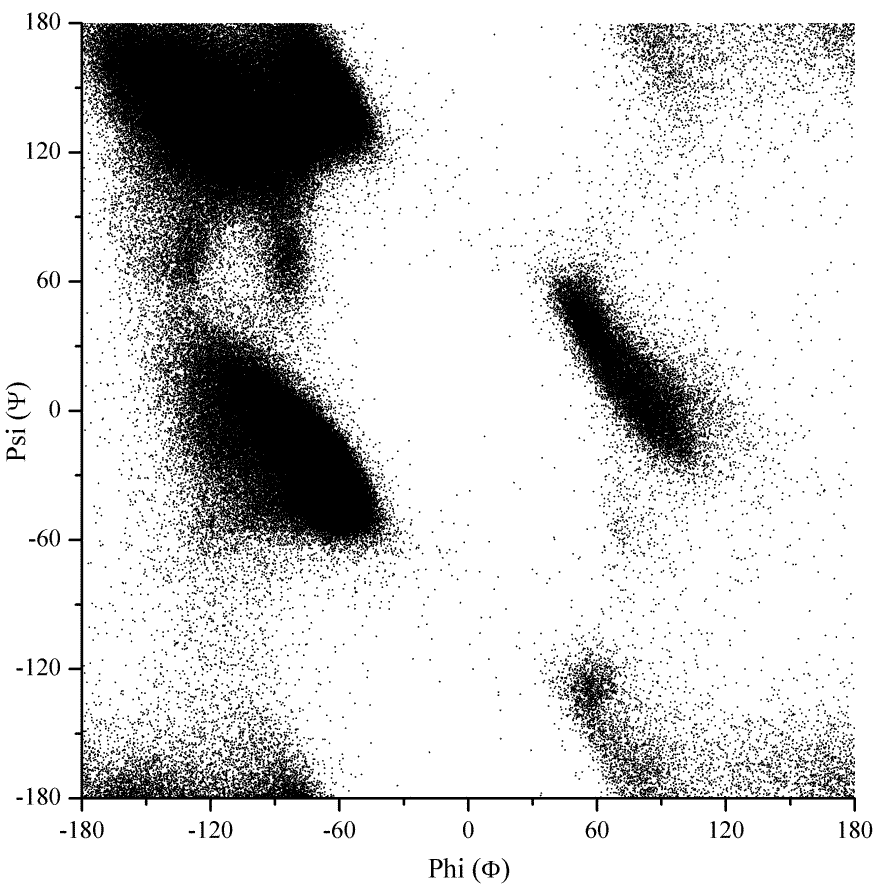
\includegraphics[width=1.0\textwidth]{./01-ProteinStructure/ramachandran/ram_scatter.png}
\end{minipage}
\hspace{0.5cm}
\begin{minipage}[b]{0.47\linewidth}
\centering
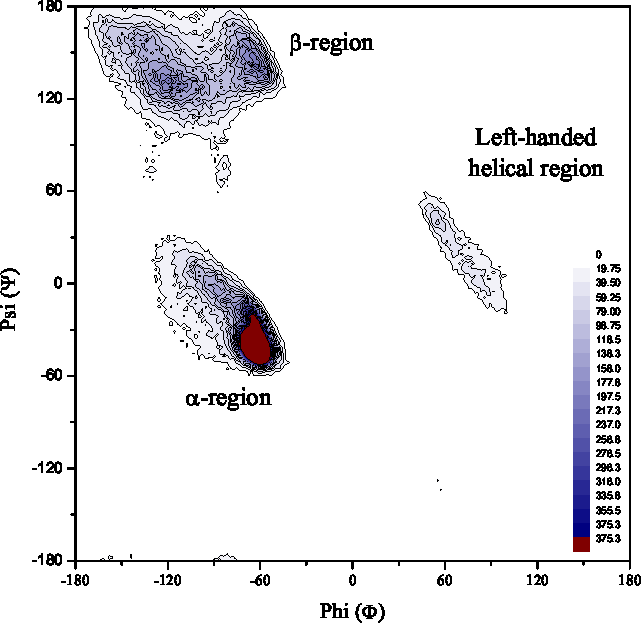
\includegraphics[width=1.0\textwidth]{./01-ProteinStructure/ramachandran/ram_Contour.pdf}
\end{minipage}
\caption[The typical Ramachandran plot]{The typical Ramachandran plot. Plotted using \xray\ crystallographic data from all non-proline and non-glycine residues from structures of \textgreater 1.8\AA\ resolution within the PDB. Left: A scatter plot. Right: A contour plot illustrating the density of data;  annotated with the class of secondary structure that each populated region represents. }
\label{fig:intro:ramachandran}
\end{figure}

A measure of structural quality can be obtained by looking at deviations from these ``ideal'' Ramachandran distributions for a given structural model, however at least mild deviations do occur in all high quality PDB structures. An individual amino acid may tolerate small local deviations from its idealised backbone torsion angles in order to optimise stabilising tertiary interactions in the protein as a whole, such as hydrogen bonding, hydrophobic burial or substrate and ligand interactions in an active site. These deviations can be clearly seen in the ``haze'' of data points around the high density idealised regions.






\subsection{Secondary Structures}

Inspection of the Ramachandran plot in figure \ref{fig:intro:ramachandran} clearly reveals three regions of extremely high propensity. These highly populated
regions represent the basic regularised secondary structural motifs of the
\ahelix, \bstrand\ and left-handed helix. The vast majority of the structure within the core of globular proteins  is described by these motifs. 


\al-helices\cite{NATIVE:Pauling1951:Helix} and \be-strands\cite{NATIVE:Pauling1951:Sheet}, shown diagrammatically in figure \ref{fig:intro:secstruc}, were originally predicted by Pauling and Corey, as early as 1951, on the grounds of geometry and hydrogen bonding alone.
The right-handed \ahelix\ is the most common form of helix in protein structure,
exhibiting 3.6 residues per turn. Critically it is the specific repeating
hydrogen bonding pattern which defines an \ahelix. Hydrogen bonds
within helices are local-sequence interactions whereby the N--H group of each participating amino acid forms a bond with the C=O group of the amino acid four residues earlier.
\bstrands\  are not  common in isolation, but instead form sheets stabilised by regular hydrogen bonding patterns. As opposed to the local bonding
interactions of helices, \bstrands\ require long-range interactions within
the polypeptide chain. \bsheets\ come in two varieties; the parallel and anti-parallel.

\begin{figure}[p]
\begin{center}
\subfigure[A typical \ahelix]{%
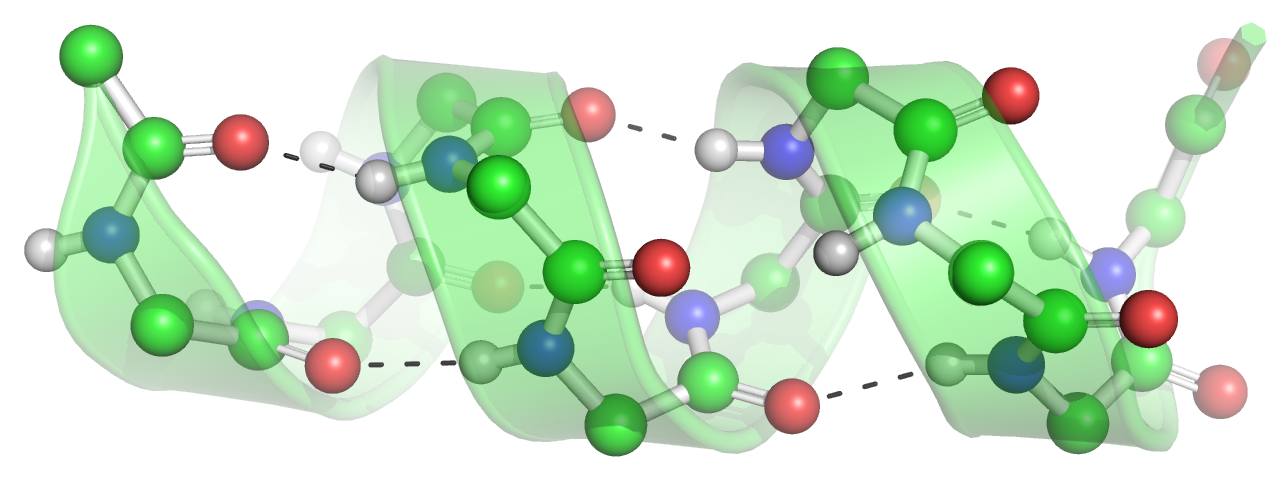
\includegraphics[width=0.8\textwidth]{./01-ProteinStructure/secstruc/helix.png}%
}
\quad
\subfigure[A typical anti-parallel \bsheet]{%
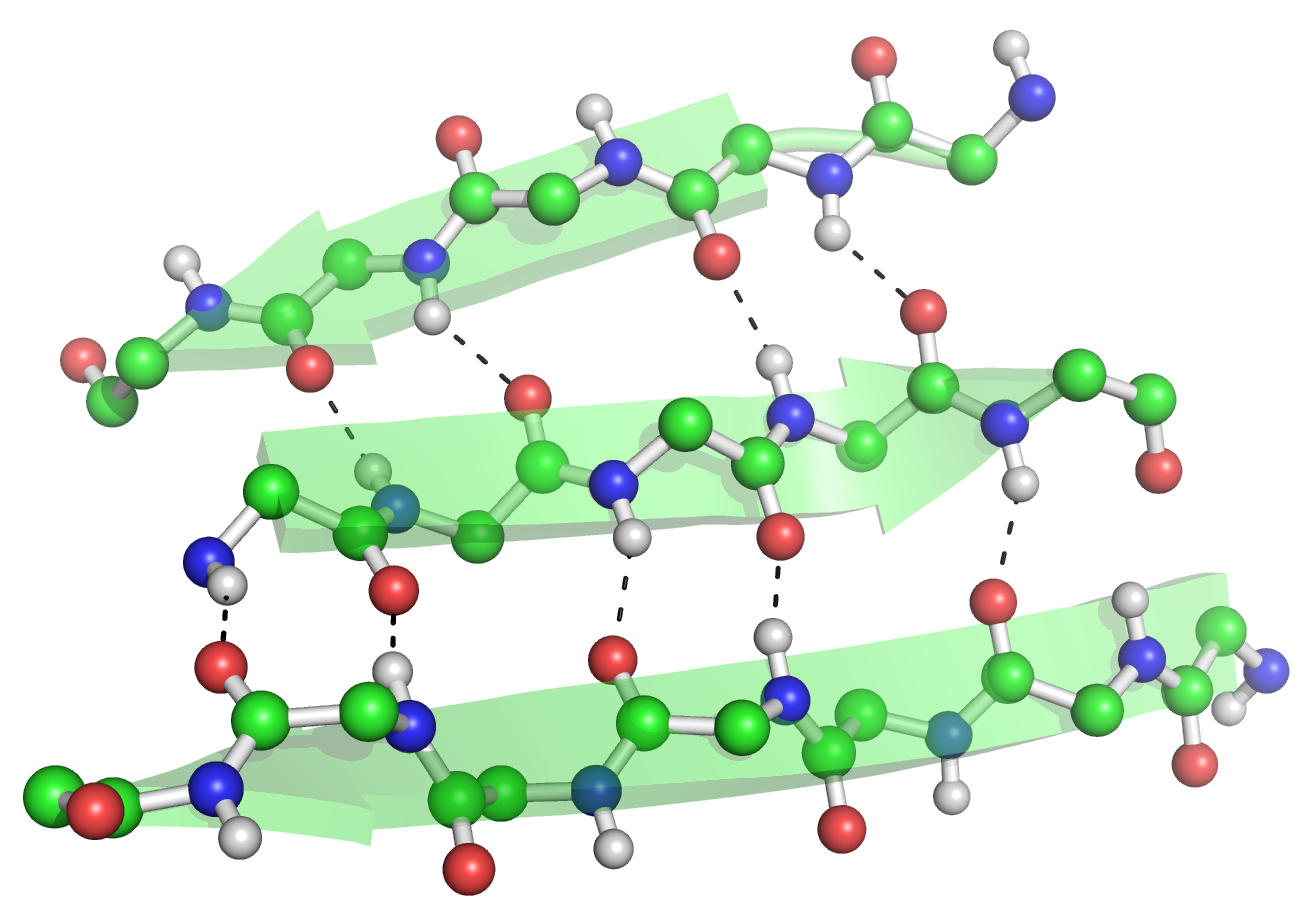
\includegraphics[width=0.8\textwidth]{./01-ProteinStructure/secstruc/antiparallel_strand.png}%
}
\quad
\subfigure[A typical parallel \bsheet]{%
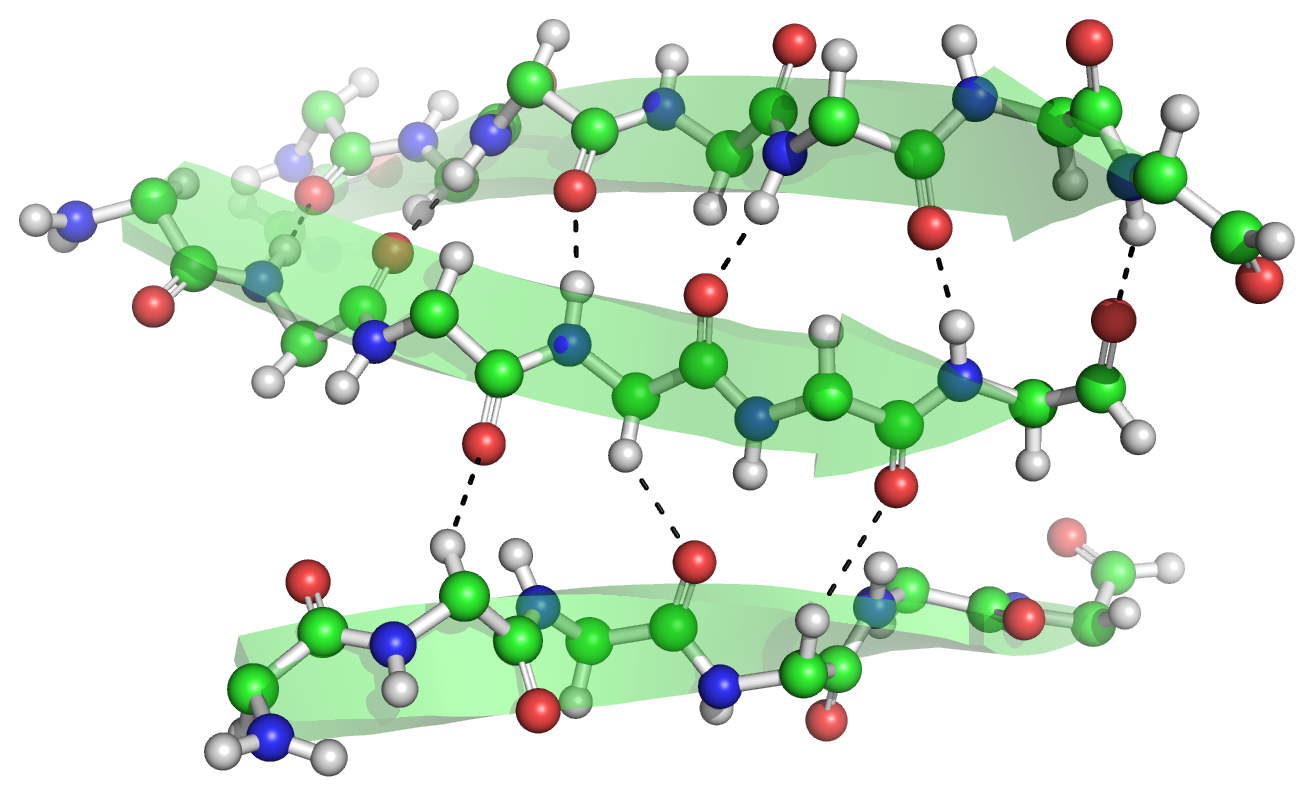
\includegraphics[width=0.8\textwidth]{./01-ProteinStructure/secstruc/parallel_strand.png}%
}
\caption[Basic secondary structure in globular proteins]{Basic secondary structure in globular proteins. Hydrogen bonds are shown as black dashed
lines. Images created using \pymolV.}
\label{fig:intro:secstruc}
\end{center}
\end{figure}

In addition to very common \al-helical and \bsheet\ structures in globular proteins, there are also other less common forms of secondary structure, as described in table \ref{table:intro:secstruc}. These include alternative helical forms
which are defined by repeating units containing different numbers of amino acids\footnote{For helical structural definitions, hydrogen bonding is defined in terms of $i$. $i \rightarrow i+x$ signifies that within a given repeat unit, the first residue forms a hydrogen bond with the residue $x$ further ahead in the primary sequence. This does not apply to \bstrands\ as their hydrogen bonding occurs between long-range
sections of the primary sequence.}. It is worth mentioning that these helices are less stable than the
\ahelix\ and are therefore typically much shorter. In all regular secondary structures, it is the  repeating pattern of hydrogen bonding that gives the
structure its stability.

\begin{table}[htbp]
\begin{center}
\begin{tabularx}{0.99\textwidth}{+l^r^r^c^X}
\toprule
\rowstyle{\bfseries}
  Name &   $\Phi$  &   $\Psi$  & Handed &  Comments \\
\midrule
  3\subscript{10}-helix   & -49 & -26 & right & Hydrogen bonded $i \rightarrow i+3$     \\
  \ahelix\                & -60 & -45 & right & Hydrogen bonded $i \rightarrow i+4$     \\
  $\pi$-helix             & -57 & -80 & right & Hydrogen bonded $i \rightarrow i+5$     \\
  Left-handed helix       &  57 &  47 &  left &                                         \\
  Type-II helices         & -79 & 150 &  left & Formed by poly-glycine and poly-proline \\
  Collagen helix          & -51 & 153 &  left & Formed by three left-handed helices     \\
\midrule
  \bstrand                &-119 & 113 &   --  & Parallel \bsheet                        \\
  \bstrand                &-139 & 135 &   --  & Anti-parallel \bsheet                   \\
\bottomrule
\end{tabularx}
\caption{The names, averaged \phipsi\ values and comments associated with the common regularised structure classifications.}
\label{table:intro:secstruc}
\end{center}
\end{table}









\subsection{Distortions in Secondary Structure }

When Pauling and Corey produced the original definitions for \ahelixs\ and \bsheets\, they were based purely upon strict geometric criteria and so made no comment
on the potential distortion of such structures. By contrast, in real proteins within the PDB
all manner of distortions in these structures can be found.  In light of
this, many examples exist where it is unclear as to whether a region should
be annotated as a regular structure, a secondary structure break or part of a surface loop structure. Within these ambiguous regions some distinct structural
motifs can be defined, which are termed secondary structure distortions.

 
\subsubsection{Helical Distortions}

Helices in real protein structures exhibit averaged \phipsi\ angles that differ slightly from those present for a textbook ideal helix. 
Of 48 analysed \ahelixs\, only 15\% are considered to be truly linear, of the remainder 17\% are kinked and 58\% are curved\cite{AUTO:HelixKinks}.

Helix curvature is generally caused by differences in hydrogen bonding geometry
on the two sides of the helix caused by carbonyl-solvent and \sidechain\ interactions on the solvent exposed helical face. This  curvature is often centred on the hydrophobic side of the helix. Overall, curvature is not expected to be energetically expensive and has been estimated at 
$<2$ \kcalmol\ for a five turn helix.

Kinks are often caused by proline residues, which are  conserved
 between homologous protein sequences, signifying their structural/functional importance. The angle of such kinks is usually of the order of 26\degree.
It is not the proline residue itself that causes the kink, as the \phipsi\
angle of proline is helical, but the  proline \sidechain\ which imposes
non-helical backbone torsions on the preceding residue. For this reason,
proline is commonly found at the start of \ahelixs.


\subsubsection{Beta-bulges} 

The $\beta$-bulge\cite{STRUCTURE:Mil87,STRUCTURE:Mil88:Bulge,STRUCTURE:Chan1993} is a small piece of non-repetitive structure that can occur by itself in loop regions, but which most often occurs as a common irregularity in anti-parallel $\beta$-structure. Almost all bulges occur at the edge of a sheet, with the
bulged strand being the outermost one. Most examples involve anti-parallel strands, with fewer than 10\% of $\beta$-bulges being between parallel strands
even though the ratio of anti-parallel to parallel $\beta$-sheets
is approximately 4.5 to 1\cite{STRUCTURE:Chan1993}. $\beta$-bulges usually occur due to the introduction of an additional residue with helical \phipsi\ angles into a \bsheet\ which causes a $\sim$10\degree\ twist. 
The two most common kinds are the Classic and G\subscript{1} bulges with other less common types, namely wide, bent and special. All $\beta$-bulge types have additional sub-types dependent on the
exact structural features.

\begin{figure}[hptb]
\begin{center}
\subfigure[A classic $\beta$-bulge from 1GL0 showing the accepted annotation of residues 1, 2 and X -- residues Phe41, Cys42 and Lys33 respectively.]{
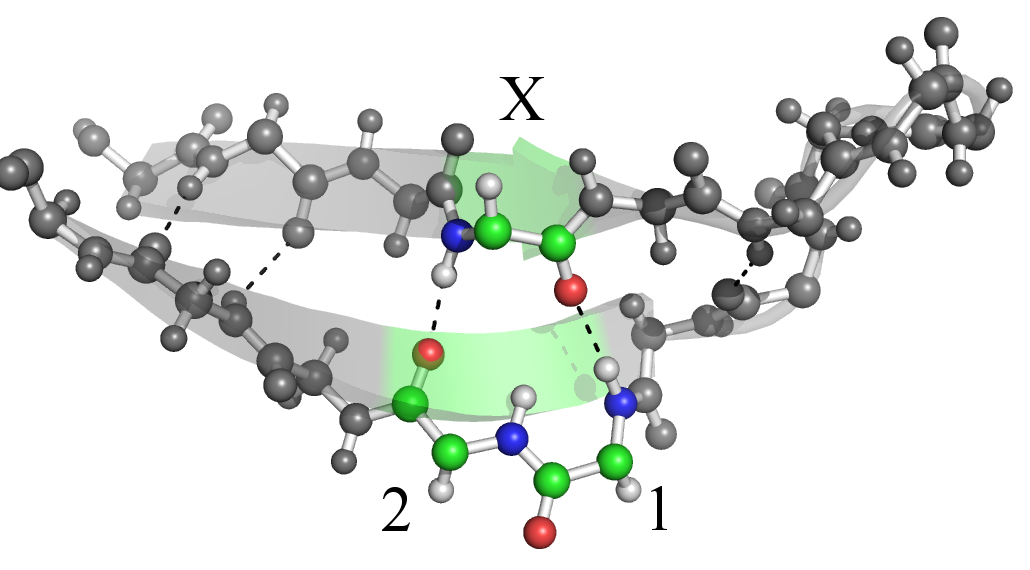
\includegraphics[width=0.8\textwidth]{01-ProteinStructure/bulges/bulge.png}
}

\subfigure[A wide $\beta$-bulge from 2ER7 showing the accepted annotation of residues 1, 2 and X -- residues Thr205, Ser206 and Thr195 respectively.]
{
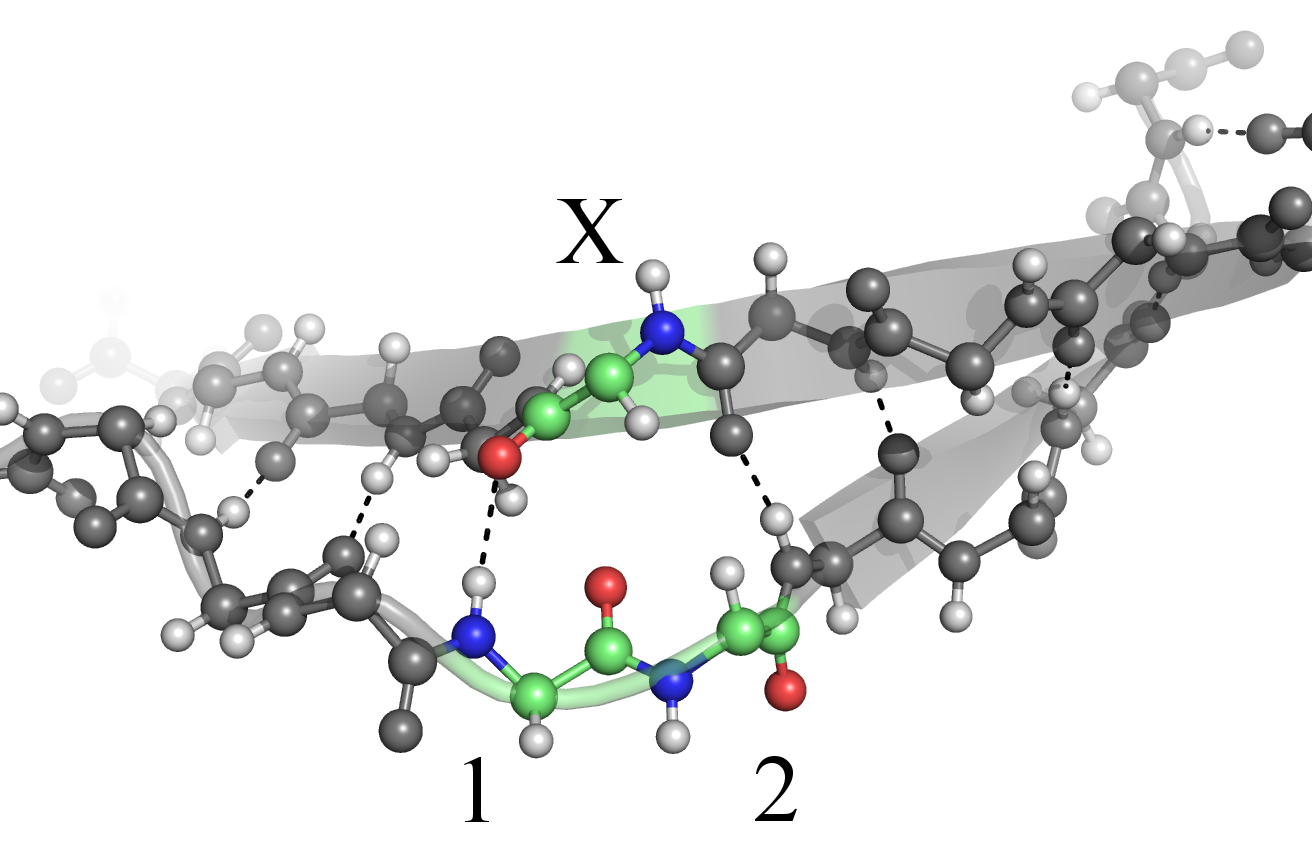
\includegraphics[width=0.8\textwidth]{01-ProteinStructure/bulges/bulge-wide.png}
}
\caption[Typical \be-bulges]{Typical \be-bulges. The classical and wide classifications
are shown. Hydrogen bonds are shown as dashed lines. Only the resides involved in the bulge itself are shown in colour.}
\label{fig:intro:bbulge}
\end{center}
\end{figure}

\begin{description} \isep

\item[Classic] $\beta$-bulges, illustrated in figure \ref{fig:intro:bbulge}-a, occur between the narrowly-spaced pair of hydrogen
bonds on anti-parallel strands. A single residue is inserted, causing the bulge. The \sidechains\ of positions 1, 2, and $X$ are all on the same side of the \bsheet. Residue 1 is in approximately $\alpha$-helical conformation and residues 2 and $X$ in approximately normal $\beta$ conformation.

\item[Wide] $\beta$-bulges, by contrast, occur between the widely-spaced pair of hydrogen bonds on anti-parallel strands. A typical example is shown
in figure \ref{fig:intro:bbulge}-b. They are apparently much less constrained than the narrow classic bulges, since they occur with a great variety of backbone conformations; they are however less common. 

\item[Special] $\beta$-bulges are the most unusual and include a G\subscript{x} sub-type, so named because they have a high propensity for glycine in position $X$.
Special bulges are defined to have between two and
four extra residues on one strand.
\item[G1] $\beta$-bulges are often observed to occur at the loop end of beta-hairpins. G1 $\beta$-bulges, defined by characteristic hydrogen bonding and dihedral angles, are sometimes found to act as a sort of turn in the absence of any adjacent anti-parallel $\beta$-hairpin.

\end{description}

$\beta$-bulges are not only of structural importance, but can also be functionally
relevant. For example, in superoxide dismutase, two bulges at the end of two functionally important loops causes them to curl away from the main $\beta$-barrel to enclose the active site\cite{STRUCTURE:Getzoff1989}. In specific cases like the Immunoglobulin-family proteins, $\beta$-bulges are conserved to aid in dimerisation of the Ig domains.
























\subsection{Loop Structure}
\label{section:loop_structure}

Mainly during the 1980s it was recognised that ``random-coil'' regions in
proteins are not, after all, completely random. Additional distinct structural motifs exist\cite{NATIVE:anatomy}, but are simply harder to categorise than regular secondary structure. It is convention to refer to shorter loops as ``simple~loops'', whereas longer loops which may contain one or more classified simple loop types are termed ``compound~loops''. 

Surface loops range in length from 1 to as many as 30 residues, although the majority are less than 12 residues in length\cite{METHOD:Fis2000}. Protein surface loops often play key functional roles and many residues are intimately involved in active sites. Some loops exhibit high structural diversity and flexibility, which may mean they are not structurally or functionally well defined\cite{METHOD:Heuser2004}.

This section describes the main classes that have been described in the literature. The knowledge of these structures should be exploited in order to make loop modelling more representative and efficient.





\subsubsection{Disallowed Regions of the Ramachandran Plot}

As has been discussed, the distribution on a Ramachandran plot shows clear bias
towards a small number of distinct \phipsi\ locations. There is however a significant
amount of data that does not occupy these regions, even in structures  which
have a high
degree of experimental confidence.
These regions  were originally referred to as
``disallowed'' in hard-sphere modelling studies performed on the protein
backbone\cite{NATIVE:Ramachandran1968}.  Recent studies however have analysed data
in these disallowed regions to see what structural motifs they relate to\cite{NATIVE:DISALLOWED,NATIVE:Gunasekaran1996}.
Other structural studies have focused on individual residues occupying specific disallowed regions\cite{NATIVE:Vega2000}. It is thought that excursions into the Ramachandran prohibited regions will usually incur a strain of at least 5 \kcalmol, in contrast to typical free energy changes for protein folding which are in the range of -5 to -15 \kcalmol\cite{NATIVE:Her91}.



In the most recent study, which focused exclusively on extremely high resolution
structures, it was found that out of a total of 63,949 non-glycine residues, only 241 (0.4\%) were found in the entirely disallowed region. Around a 70\% majority of residues located in disallowed regions are solvent-exposed, indicating
a vastly increased importance in loop structure\cite{NATIVE:DISALLOWED}. It is important to note that although a low proportion of residues exist in a disallowed region, around 3\%, 6\%
and 8\% short and medium and long length loops respectively do have at least one residue in a disallowed region (section \ref{section:loop_stats}). 

These large deviations from allowed Ramachandran regions, which cannot be ascribed to experimental error, are usually found exhibiting compensating interactions. The loss of hydrogen bonding is less important at the protein surface compared to the protein core due to solvation effects.
However, \sidechain\ or non-regular hydrogen bonds, are often be involved and many are described throughout the remainder of this section. 

Figure \ref{fig:intro:disallowed} shows clustered disallowed  regions. Clusters II and III normally correspond to residues which are stabilised by hydrogen bonds in turns. Residues in cluster I are sometimes stabilised by \sidechain\ hydrogen bonding and occur as part of distorted \bstrands. Cluster IV is found in some unusual conformations, one example of which involves a tyrosine residue \sidechain\ interaction.\ In this example, the aromatic face of the \sidechain\ was involved in a C--H $\to$ $\pi$-orbital interaction and a hydrogen bond was formed by the terminal oxygen\cite{NATIVE:Sam2000}. Cluster V can be considered to be an extension of the beta region -- a nomenclature artefact produced by the original definition of the \be-region in the original disallowed region study\cite{NATIVE:Gunasekaran1996}.
 
\begin{figure}[hptb]
\vspace{0.4cm}
\begin{minipage}[b]{0.47\linewidth} % 0.5 for half the page
\centering
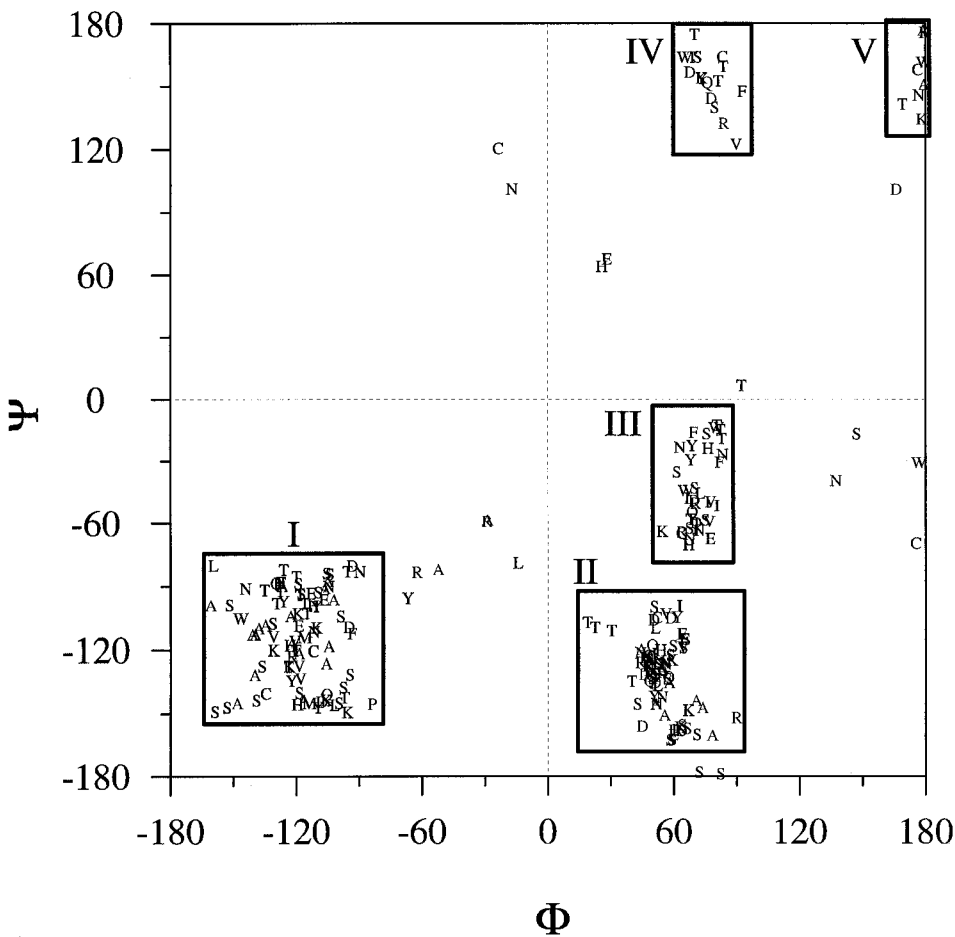
\includegraphics[width=1.0\textwidth]{01-ProteinStructure/ramachandran/disallowed.png} % 1.0 to take ALL the half page
\end{minipage} 
\hspace{0.4cm} % To get a little bit of space between the figures
\begin{minipage}[b]{0.47\linewidth} % 0.5 for half the page
\centering
\begin{small}
\begin{tabularx}{1.0\textwidth}{+c^X}
\toprule
\rowstyle{\bfseries} Cluster & Residue Preference \\
\midrule
 I & Ser, Pro (low incidence) \\
 II & Ser, Asp, Asn, Polar and Leu \\
 III & Ser, Aromatic, not Ala, Ile (low incidence)  \\
 IV & Ser, Aromatic, not Ala  \\
\bottomrule
\end{tabularx}
\end{small}
\caption[Disallowed regions of the Ramachandran map.]{Disallowed regions of the Ramachandran map in 363 high resolution chains. (Figure adapted from\cite{NATIVE:DISALLOWED}.)}
\label{fig:intro:disallowed}
\end{minipage}
\end{figure}

Conformational analysis reveals that for these disallowed regions and also cis-containing peptides\cite{NATIVE:Her91} there are actually relatively few sterically strained features present. Those steric infringements that do occur are located overwhelmingly in regions concerned with function, which is most likely due to the greater precision necessary for ligand binding and catalysis, compared with the requirements of satisfactory folding. 








\subsubsection{Tight-Turns}
\label{section:intro:tightturns}

Tight-turns are abundant in globular proteins and were recently reviewed\cite{STRUCTURE:Cho2000}. A tight-turn in protein structure is defined as a site of no more than six residues where the polypeptide chain reverses and folds back on itself by around 180\degree. The peptide concerned must not be in a helical conformation. A turn formed by seven or more amino acids is not considered as a tight-turn, but rather as a ``loose turn''. The classes of tight-turns are categorised by loop length -- $\delta$-turn\cite{STRUCTURE:Ton80}, $\gamma$-turn\cite{STRUCTURE:Nem72,STRUCTURE:Mil88}, $\beta$-turn\cite{STRUCTURE:Mil86,STRUCTURE:Mil87,STRUCTURE:Hut94}, $\alpha$-turn\cite{STRUCTURE:Ton80,STRUCTURE:Pav96}, and $\pi$-turn\cite{STRUCTURE:Raj96,STRUCTURE:Kim76} -- which are formed by two, three, four, five, and six amino acid residues respectively. 

Tight-turns usually exhibit the following
features: 
\begin{enumerate} \isep
\item A distance between the \ca\ atoms of the first and last residue of $<$7\AA.\
\item In most cases an intra-turn hydrogen bond between the backbone oxygen of the first residue and backbone nitrogen of the last residue is present.
\item Multiple populated trajectories to reverse the chain direction as reflected by distinct preferred residue types at each position and characteristic backbone dihedral angles of the inner residues.
\end{enumerate}

\paragraph{$\delta$-turns} \isep
Of the tight-turn classes, the smallest is a $\delta$-turn involving only two amino acid residues. It is categorised by 1$\rightarrow$2 type, 2$\rightarrow$3 type, or C\subscript{8} form. The intra-turn hydrogen bond for a $\delta$-turn is formed between the backbone atoms NH\subscript{(i)} and CO\subscript{(i+1)}. 

\paragraph{$\gamma$-turns} \isep
$\gamma$-turns involve three residues and a hydrogen bond between the backbone atoms CO\subscript{(i)} and NH\subscript{(i+2)}. Residues in the $i$+1 position of a $\gamma$-turn are partly responsible for disallowed cluster 3 -- the $\Phi$=80\degree\, $\Psi$=-70\degree\ region of the Ramachandran plot \mbox{(figure \ref{fig:intro:disallowed})}. The typical averaged \phipsi\ values for this residue position have been analysed and the two main classes named (table \ref{table:intro:gammaturn}).

\begin{table}[hptb]
\begin{small}
\begin{center}
\begin{tabular}{+l^r^r}
\toprule
\rowstyle{\bfseries}
  Type &  $\mathbf{\Phi^{\circ}_{\mathbf{(i+1)}}}$ &   $\mathbf{\Psi^{\circ}_{\mathbf{(i+1)}}}$ \\
\midrule
  Classic $\gamma$-turn           & \color{red}{75} & \color{red}{-64} \\
  Inverse $\gamma$-turn           & -79 &  69 \\
\bottomrule
\end{tabular}
\caption[Possible $\gamma$-turn \phipsi\ angles]%
{Possible $\gamma$-turn \phipsi\ angles.
Residues occupying disallowed Ramachandran space are listed in red.
(Data \cite{STRUCTURE:Nem72}.)}
\label{table:intro:gammaturn}
\end{center}
\end{small}
\end{table}



\paragraph{$\beta$-turns} \isep
Perhaps the best-characterised and described class of turn is the $\beta$-turn. The $\beta$-turn has a long history of being re-categorised
with significant debate over the poorly represented classes.
Classification was originally defined based on \phipsi\ torsions in three distinct conformational classes and their \ca\ mirrors; types I, II, III and I', II', III' respectively\cite{STRUCTURE:Ven1968}.
As more structural information emerged the classes were expanded to ten types \cite{STRUCTURE:Lew73} and then reduced to just six types with a miscellaneous ``catch-all'' class to cover outliers\cite{NATIVE:anatomy}. In the most recent studies involving significantly more data, eight defined classes are used along with the miscellaneous class\cite{STRUCTURE:Hut94,STRUCTURE:Wilmot1990}.
Examples of these turn types are shown in figures \ref{fig:intro:bturn1} and \ref{fig:intro:bturn2} which are derived from the PDB structures in table \ref{table:intro:bturn_chains}. The \phipsi\ data is shown in Table \ref{table:intro:betaturn}.

\begin{figure}[p]

\begin{minipage}[b]{0.5\linewidth}
\centering
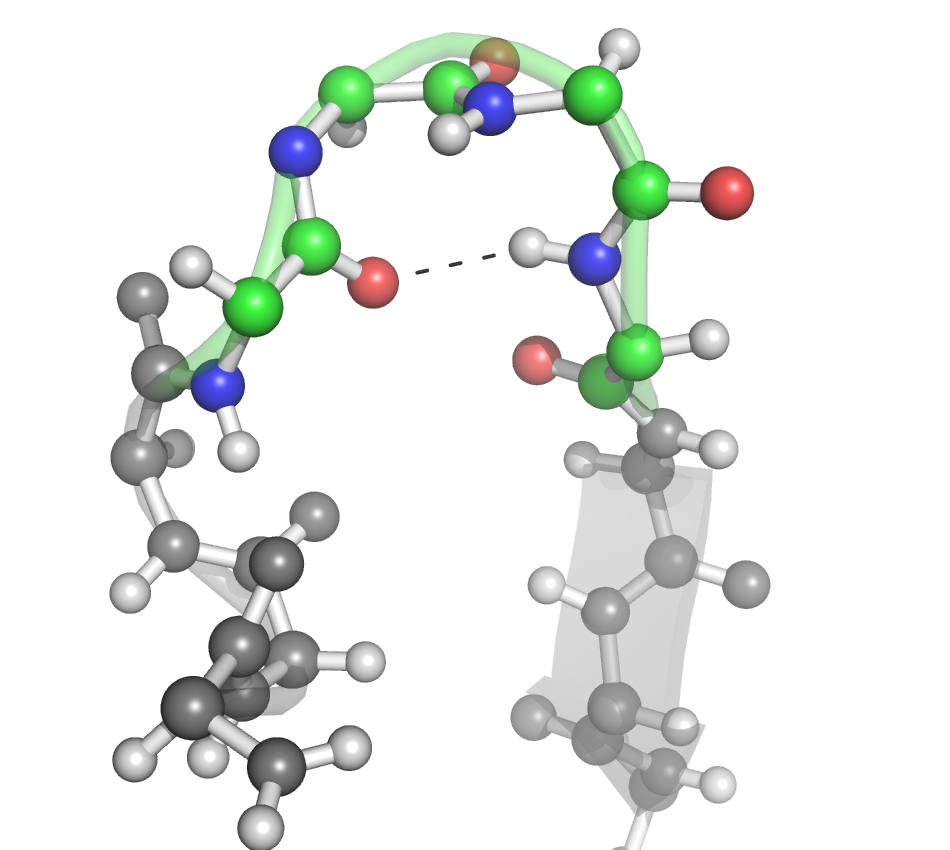
\includegraphics[width=1.0\textwidth]{./01-ProteinStructure/turns/beta-type-I.png}
\end{minipage}
\hspace{0.5cm}
\begin{minipage}[b]{0.3\linewidth}
\centering
Type I
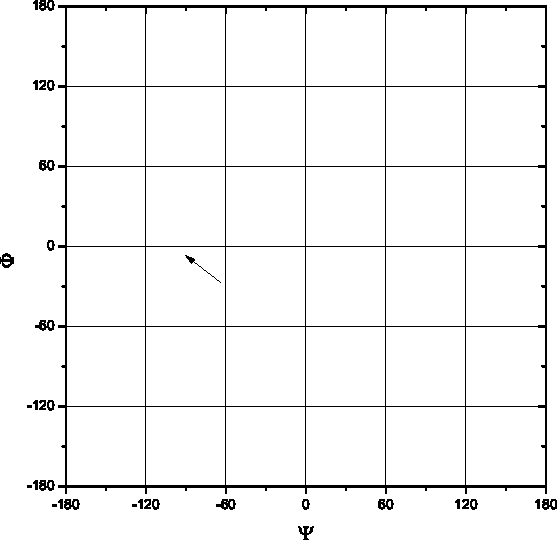
\includegraphics[width=1.0\textwidth]{./01-ProteinStructure/turns/beta-ram-type-I.pdf}
\end{minipage}

\begin{minipage}[b]{0.5\linewidth}
\centering
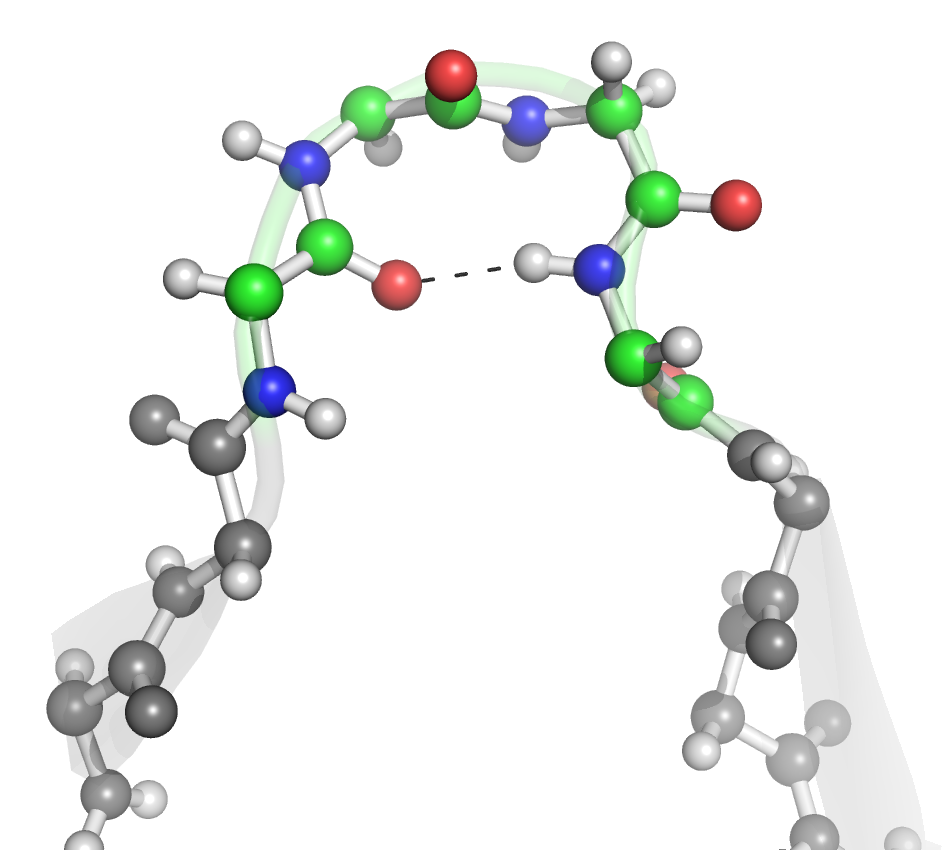
\includegraphics[width=1.0\textwidth]{./01-ProteinStructure/turns/beta-type-II.png}
\end{minipage}
\hspace{0.5cm}
\begin{minipage}[b]{0.3\linewidth}
\centering
Type II
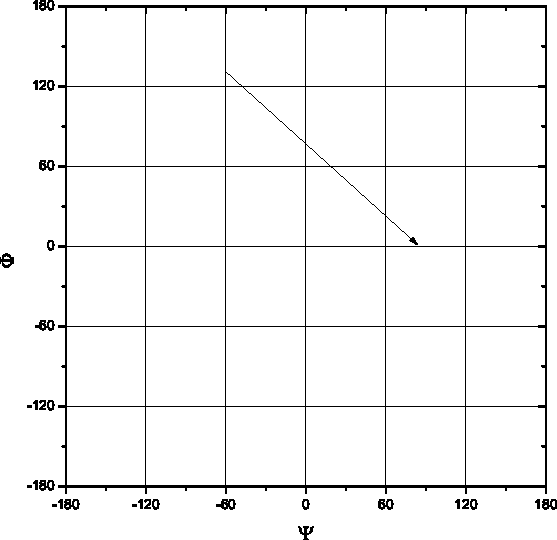
\includegraphics[width=1.0\textwidth]{./01-ProteinStructure/turns/beta-ram-type-II.pdf}
\end{minipage}

\begin{minipage}[b]{0.5\linewidth}
\centering
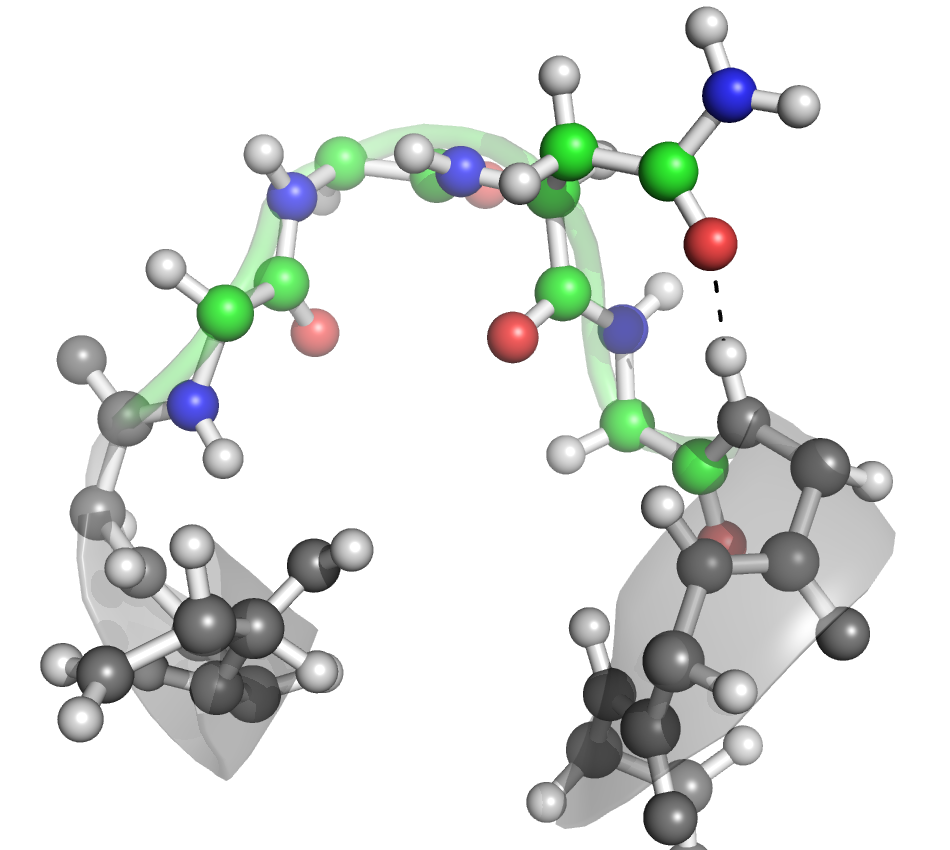
\includegraphics[width=1.0\textwidth]{./01-ProteinStructure/turns/beta-type-VIII.png}
\end{minipage}
\hspace{0.5cm}
\begin{minipage}[b]{0.3\linewidth}
\centering
Type VIII
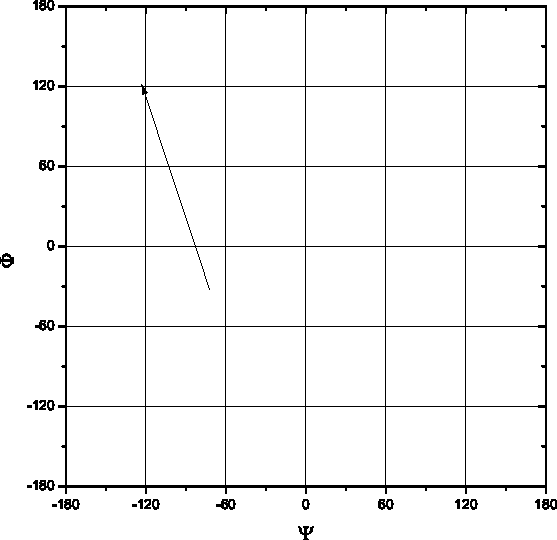
\includegraphics[width=1.0\textwidth]{./01-ProteinStructure/turns/beta-ram-type-VIII.pdf}
\end{minipage}

\caption[$\beta$-turns of class I, II and VIII]{$\beta$-turns of class I, II and VIII: Types I and II are the most common classical types. Non-classical
type VIII turns show no
intra-chain hydrogen bond, but are stabilised instead by a \sidechain$\rightarrow$backbone hydrogen bond. Ramachandran plots are presented showing residues $i$+1 and $i$+2.}
\label{fig:intro:bturn1}

\end{figure}

\begin{figure}[p]

\begin{minipage}[b]{0.5\linewidth}
\centering
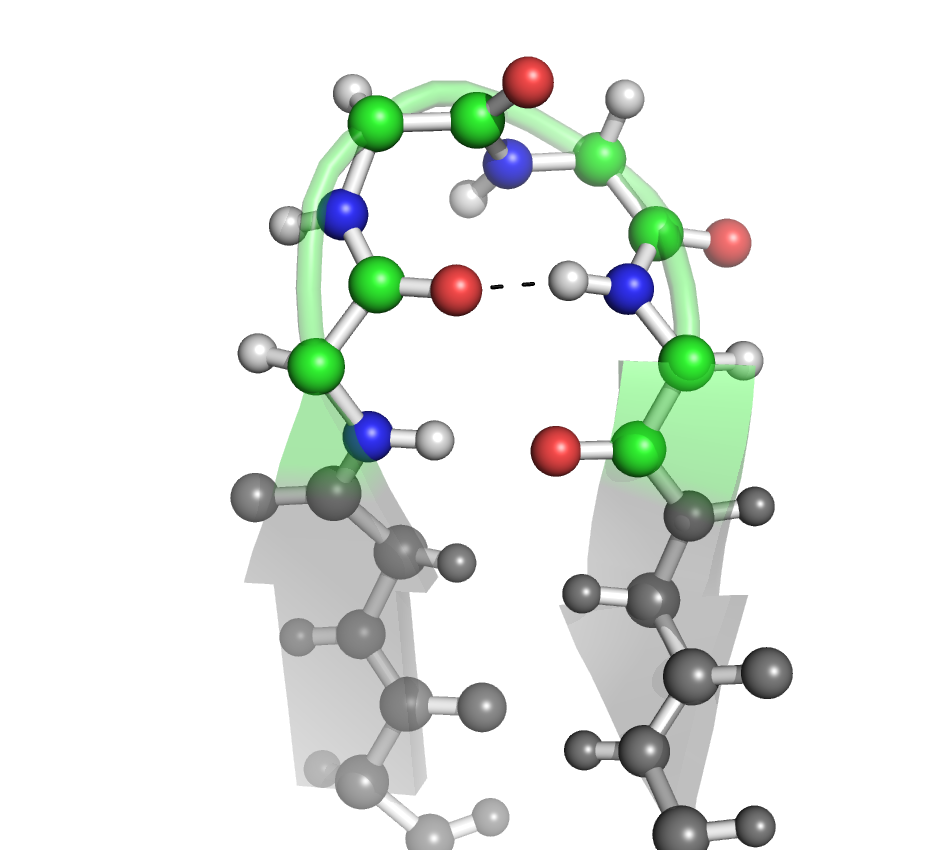
\includegraphics[width=1.0\textwidth]{./01-ProteinStructure/turns/beta-type-Ip.png}
\end{minipage}
\hspace{0.5cm}
\begin{minipage}[b]{0.3\linewidth}
\centering
Type I'
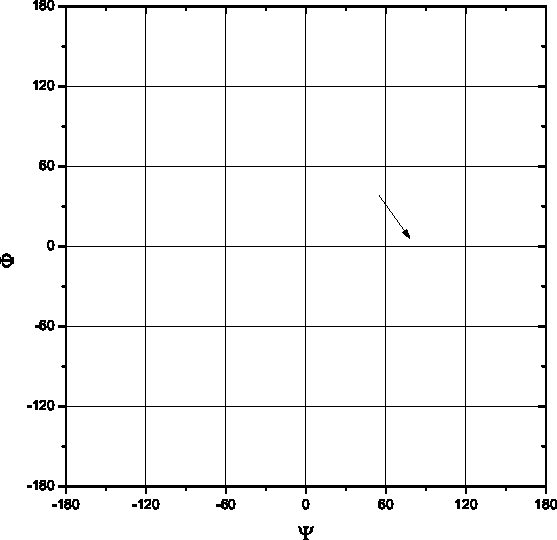
\includegraphics[width=1.0\textwidth]{./01-ProteinStructure/turns/beta-ram-type-Ip.pdf}
\end{minipage}

\begin{minipage}[b]{0.5\linewidth}
\centering
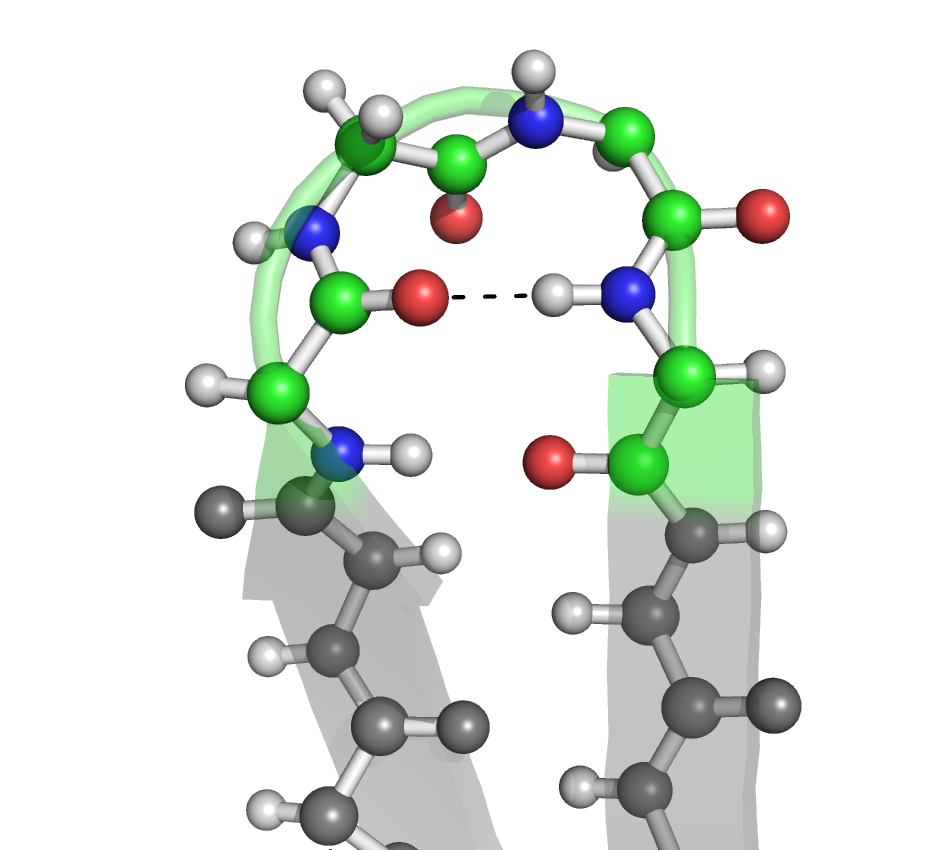
\includegraphics[width=1.0\textwidth]{./01-ProteinStructure/turns/beta-type-IIp.png}
\end{minipage}
\hspace{0.5cm}
\begin{minipage}[b]{0.3\linewidth}
\centering
Type II'
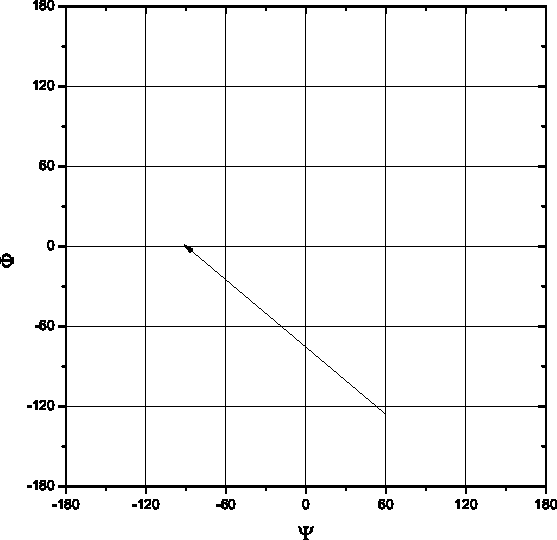
\includegraphics[width=1.0\textwidth]{./01-ProteinStructure/turns/beta-ram-type-IIp.pdf}
\end{minipage}

\caption[$\beta$-turns of class I' and II']{$\beta$-turns of class I' and II':
These are common classical turns involved in $\beta$-hairpins. Ramachandran plots are presented showing residues $i$+1 to $i$+2.}
\label{fig:intro:bturn2}

\end{figure}

\begin{table}[p]
\begin{small}
\begin{center}
\begin{tabular}{+c^c^c^c}
\toprule
\rowstyle{\bfseries}
  Type & PDBID & Residues & Sequence \\
\midrule
  I    & lCSE & 39-42   & HPDL \\
  II   & 1AAC & 38-41   & KVGD \\
  VIII & 1LZ1 & 86-90   & QDNI \\
  I'   & 1CGT & 293-296 & KDGA \\
  II'  & 1BBT & 19-22   & NGHT \\  
\bottomrule
\end{tabular}
\caption{PDB chains used in the $\beta$-turn figures \ref{fig:intro:bturn1} and \ref{fig:intro:bturn2}.}
\label{table:intro:bturn_chains}
\end{center}
\end{small}
\end{table}

\begin{table}[hbtp]
\begin{small}
\begin{center}
\begin{tabular}{+l^c^r^r^r^r^l}
\toprule
\rowstyle{\bfseries}
  $\beta$-turn & Plot\superscript{*}\ &
  $\mathbf{\Phi^{\circ}_{\mathbf{(i+1)}}}$ & $\mathbf{\Psi^{\circ}_{\mathbf{(i+1)}}}$
  &
  $\mathbf{\Phi^{\circ}_{\mathbf{(i+2)}}}$ & $\mathbf{\Psi^{\circ}_{\mathbf{(i+2)}}}$
  &
  Comment \\  
\midrule
I     & $\alpha_R\alpha_R$ &  -64  &  -27 &  -90 &  -7 & Most common type \\
II    & $\beta\gamma_L$    &  -60  &  131 &   84 &   1 & Common type \\
VIII  & $\alpha_R\beta$    &  -72  &  -33 & -123 & 121 & Common non-classic\\
I'    & $\alpha_L\gamma_L$ &   55  &   38 &   78 &   6 & Forms $\beta$-hairpins \\
II'   & $\epsilon\alpha_R$ & {\color{red}{60}}  & {\color{red}-126} &  -91 &   1 & Forms $\beta$-hairpins \\
VIal  & $\beta\alpha_R$    &  -64  &  142 &  -93 &   5 & --\\
VIa2  & $\beta\alpha_R$    & -132  &  139 &  -80 & -10 & --\\
VIb   & $\beta\beta$       & -135  &  131 &  -76 & 157 & --\\
IV    & --                  &  -61  &   10 &  -53 &  17 & Miscellaneous class\\
\bottomrule
\end{tabular}
\caption[$\beta$-turn classes and corresponding averaged \phipsi\ angles]{$\beta$-turn classes and corresponding averaged \phipsi\ angles.
Residues occupying disallowed Ramachandran space are listed in red. (Data\cite{STRUCTURE:Hut94} and Ramachandran plot nomenclature\superscript{*}\cite{STRUCTURE:Wilmot1990}.)}
\label{table:intro:betaturn}
\end{center}
\end{small}
\end{table}

Types I and II are the most common \be-turns, the essential difference between them being the orientation of the peptide bond between residues at $i$+1 and $i$+2. Most exhibit a hydrogen bond from the backbone atoms CO\subscript{(i)} to NH\subscript{(i+3)} which compensates for any unfavourable \vdw\ contact.

$\beta$-hairpins are a special case which occur when an extended strand reverses direction to
form two \bstrands\ hydrogen bonded to each other with a $\beta$-turn in-between.
A classification scheme for whole $\beta$-hairpins has been defined\cite{STRUCTURE:Mil86}.
The $\beta$-turn itself is restricted to a limited number of conformations\cite{STRUCTURE:Sib85,STRUCTURE:Sib89} with specific backbone torsion angles. The turn shows a distinct preference for the Type I' and Type II' conformations, which is thought to be as a consequence of compatibility of the twist of the turn with the natural right-handed twist of the beta-sheet\cite{STRUCTURE:Sib89}.

Figures \ref{fig:intro:bturn1} and \ref{fig:intro:bturn2} show typical structures
and typical \phipsi\ values on associated Ramachandran maps. Residue $i$+2
of type II $\beta$-turns is nearly always glycine as any \sidechain\
would yield steric contacts with the carbonyl oxygen of the preceding residue.
For both type I' turns at residue $i$+2 and type II' turns at residue $i$+1 glycine is almost always present, again due to steric considerations. Rarely, however, other residues can occur at these positions -- for example many of the non-glycine residues in disallowed cluster 2 of the Ramachandran map ($\Phi$=60\degree\ $\Psi$=-120\degree).  There is an energetic penalty for residues to adopt this conformation which is normally resolved by a strong \sidechain\ interaction.

\paragraph{$\alpha$-turns} \isep 
An $\alpha$-turn involves five residues where the distance between \ca$i$ and \ca$i$+4 is less than 7\AA\ and the penta-peptide chain is not in a helical conformation. The most systematic study\cite{STRUCTURE:Pav96} of $\alpha$-turn topology to date was based on structural clustering. A categorisation of nine different types based on the backbone dihedral angles of residues $i$+1, $i$+2, and $i$+3 was developed in the study. The representative \phipsi\ values for these classes are given in Table \ref{table:intro:alphaturn}. $\alpha$-turns mainly exhibit hydrophilic amino acids, meaning that these structures are not only often highly exposed to solvent, but also protrude outward from the protein surface with a ``hook-like'' shape. These structural motifs can often therefore function in protein interaction mechanisms\cite{STRUCTURE:Art81,STRUCTURE:Sto89,STRUCTURE:Wan90}.

\begin{table}[htbp]
\begin{small}
\begin{center}
\begin{tabular}{+l^r^r^r^r^r^r}
\toprule
\rowstyle{\bfseries}
  Cluster & 
  $\mathbf{\Phi^{\circ}_{\mathbf{(i+1)}}}$ & $\mathbf{\Psi^{\circ}_{\mathbf{(i+1)}}}$ &
  $\mathbf{\Phi^{\circ}_{\mathbf{(i+2)}}}$ & $\mathbf{\Psi^{\circ}_{\mathbf{(i+2)}}}$ &   
  $\mathbf{\Phi^{\circ}_{\mathbf{(i+3)}}}$ & $\mathbf{\Psi^{\circ}_{\mathbf{(i+3)}}}$ \\
\midrule
   I-$\alpha_\mathrm{RS}$ & -60$\pm11$ & -23$\pm13$ & -72$\pm14$ & -29$\pm15$ & -96$\pm20$ & -20$\pm17$\\
   I-$\alpha_\mathrm{LS}$ &  \color{red}{48$\pm22$} & \color{red}{-42}$\pm14$ &  67$\pm~9$ &  33$\pm14$ &  70$\pm11$ &  32$\pm12$\\
  II-$\alpha_\mathrm{RS}$ & -59$\pm10$ & 129$\pm15$ &  88$\pm15$ & -16$\pm19$ & -91$\pm22$ & -32$\pm18$\\
  II-$\alpha_\mathrm{LS}$ &  \color{red}{53$\pm15$} &\color{red}{-137$\pm25$} & -95$\pm12$ &  81$\pm23$ &  57$\pm~5$ &  38$\pm~8$\\
   I-$\alpha_\mathrm{LU}$ & -61$\pm12$ & 158$\pm15$ &  64$\pm17$ &  37$\pm21$ &  62$\pm12$ &  39$\pm~8$\\
   I-$\alpha_\mathrm{RU}$ &  \color{red}{59$\pm18$} &\color{red}{-157$\pm31$} & -67$\pm17$ & -29$\pm20$ & -68$\pm12$ & -39$\pm12$\\
  II-$\alpha_\mathrm{LU}$ & -65$\pm15$ & -20$\pm15$ & -90$\pm17$ &  16$\pm44$ &  86$\pm18$ &  37$\pm27$\\
  II-$\alpha_\mathrm{RU}$ &  54$\pm~8$ &  39$\pm15$ &  67$\pm13$ &  -5$\pm31$ &-125$\pm11$ & -34$\pm32$\\
   I-$\alpha_\mathrm{C}$  &-103$\pm23$ & 143$\pm4 $ & -85$\pm~8$ &   2$\pm~6$ & -54$\pm~6$ & -39$\pm~9$\\
\bottomrule
\end{tabular}
\caption[Possible $\alpha$-turn \phipsi\ angles]%
{Possible $\alpha$-turn \phipsi\ angles. Residues occupying disallowed Ramachandran space are listed in red. (Data \cite{STRUCTURE:Pav96}.)}
\label{table:intro:alphaturn}
\end{center}
\end{small} 
\end{table}


\subsubsection{Additional classifications}

\paragraph{$\Omega$-loops} first described in 1986\cite{STRUCTURE:Les86}, are a sub-set of loops characterised by a distinct shape. Being at least six residues in length, the ends of the $\Omega$-loop are close in Cartesian space. In an attempt to distinguish between $\Omega$-loops and the other simple loop types the number of residues was set between 6 and 16, with the distance between the end termini to a maximum of 10\AA\ and less than two thirds of the longest \ca$\rightarrow$\ca\ distance in the loop. Backbone torsions found in $\Omega$-loops are mostly from the highly populated Ramachandran regions, albeit by definition they do not contain repeating \phipsi\ angles or regular patterns of hydrogen bonding; many $\Omega$-loops do, however, contain a large number of \sidechain\ hydrogen bonds. It has become clear that $\Omega$-loops are often involved in protein function and molecular recognition, but those with a higher than average number of hydrogen bonds or hydrophobic contacts may play roles in protein stability and folding\cite{STRUCTURE:Fet95}. 

\paragraph{Long-loops} are defined as those containing more than ten residues. The most recent categorisation\cite{STRUCTURE:Mar95}  contains two sub-sets, the first of which is termed ``long-open'' and the second less abundant type termed ``long-closed''. The two classes are based on the distance between the ends of the loop and the nature of the of adjoining secondary structure.

\paragraph{$\alpha\alpha$-hairpins,} also known as $\alpha\alpha$-turns, have also been described in the literature\cite{STRUCTURE:Efi91,STRUCTURE:Win96}. They are defined as short connecting regions which join two \ahelixs\ together, where it was shown that each given type had very similar patterns of hydrophobic, hydrophilic and glycine residues in their respective sequences. Multiple classes have been defined, determined by the number of residues involved in the turn, defined as between one and five in the original work.

\paragraph{Generalised Languages} have been produced with the aim of describing
all loop structures.
Most notably, one definition\cite{STRUCTURE:Rin92} focuses upon the linearity and planarity of loops, proposing three global kinds called $\Omega$-loops, $\zeta$-loops, and strap-loops. Out of 432 loops (from 4 to 20 residues in length) extracted from 67 proteins, 205 were classified as linear (straps), 133 as non-linear and planar ($\Omega$) and 86 as non-linear or non-planar ($\zeta$). The classification system (as most are) was, however, imperfect as eight loops were classified as compound loops, because they contained a combination of strap, $\Omega$, and $\zeta$ morphologies.





\section{Concluding Remarks}

Most of the less well defined structural classifications are annotated primarily based upon human classification, sometimes arbitrarily, using known high-resolution protein structures. What is undisputed, however, is that many of the stronger structural
motifs have distinct \phipsi\ and residue preferences. It is, therefore, important to
keep these motifs in mind when undertaking protein modelling. Finally, it is critical
that each different residue type is treated independently in the modelling process, as it is clear that local sequence-specific effects are prevalent in globular protein structure. This is particularly true in tight turns where  \sidechain\
hydrogen bonds play an important role in backbone stabilisation.\ 
